\documentclass[10pt,fullpage]{article}

\usepackage{amsmath,amssymb,amsthm,amsfonts} % Typical maths resource packages
\usepackage{graphicx}
\usepackage{hyperref}                 % For creating hyperlinks in cross references

\makeindex

\title{The FastMatrix class}

\begin{document}
\maketitle

\section{Introduction}
The FastMatrix class is a math-oriented template C++ class for
storing arbitrary-sized matrices of arbitrary numeric type (64-bit
double precision floating point numbers are used by default to
represent real entries). fastMAtrix may also be instantiated with
other types such as complex numbers. The goal of the fastMatrix
class is to offer a number of common mathematical operations in a
reasonably efficient manner.

Internally, the matrix is stored as a random access one-dimensional
array of numbers on the heap, in row major order. Public interfaces
hide this representation and provide mathematical abstraction.

The operators $(row,col), *, +, -, =, ==$ have been overloaded to
provide a natural interface to the programmer. Other arithmetic
binary operators including  $<,
>, \ll, $ have no meaning for matrices, so they have not been
considered for overloading. As a special case, $\%$ has been
overloaded for convenient representation of a vector cross-product.

\newpage

\section{Version History}

\begin{itemize}
\item[0.0.1] Initial revision. Includes Matrix multiplication for same dimension matrices,
member-scalar operations, destructive LU decomposition without
pivoting, random access indexing, shallow copy operations, and
input/output routines.
\item[0.2.0] Includes non-interruptive standard error debugging, matrix multiplication with resizing,
matrix-matrix addition and subtraction, vector-vector operations,
vector inner-product, vector normalization, scalar division, row and
column extraction, row and column assignment, deep copy constructor,
deep copy assignment, transposition, random access indexing, copy
operations, output formats for MAPLE, MATLAB, LATEX, and CSV
tabulated spreadsheet, automated generation of special matrices such
as Fourier, Vandermonde, Identity, etc.
\item[0.2.1] Orthogonalization and test, via Gram Schmidt method and
Householder reflections, array constructor for building
block-diagonal and block-tridiagonal matrices.
\item[NEXT] Next revision will include full support for complex entries.
Revision could possibly include LU decomposition with partial
pivoting, determinants, extraction of eigenvalue / eigenvector
pairs, Orthogonalization via Givens rotations, discrete fourier
transform, etc. But it will probably just do FFTs.
\end{itemize}

\newpage

\section{Getting started}

To create a fastMatrix you must include the header file. Put it in
the local directory or a subdirectory of your current project.

\begin{verbatim}
#include "fastMatrix.h"
\end{verbatim}

The class compiles on g++ 3.4.4 and minGW 3.7. A makefile is
provided for unix systems. See the README file for up to date
information about compiling and linking.

\subsection {Example: Working with files}

The following driving code reads a sample $3x3$ matrix from the file
basic.txt. It then computes an LU factorization, creates two new
matrices $L$ and $U$, and writes them to disk as text files.

\begin{verbatim}
 typedef fastMatrix <double> matrix; //double precision numbers

 matrix A("basic.txt"); //you can also load a predefined matrix

 A.LUFactor();
 bm.clockit();

 matrix L = A.lower();
 matrix U = A.upper();
 matrix B = L*U;          //use this to check our result is valid (only for nonsingular)

assert(A == B);
//if these two are not the same then there is a problem
//the matrix is possibly nonsingular

 L.write("basic_L.txt");
 U.write("basic_U.txt");

 B.write("basic_result.txt");
\end{verbatim}

\newpage

\subsection {Example: Benchmarking}

The following sample program creates a random-valued

WARNING: This random matrix is not guaranteed to be nonsingular or
well conditioned, so the probability of the result of LU
decomposition or Gaussian elimination is less likely to be correct
as the dimension of the matrix increases.

\begin{verbatim}
 int n;
 cout << "Enter (single) dimension for random square matrix. ";
 cin >> n;
 srand(time(0));

 fastMatrix A(n, n);

 A.write("random1.txt");

fastMatrix B = A;

 bench bm("LU-Decomposition operations only"); //title our benchmark
 A.registe(&bm); //associate benchmark with the LU decomposition

 A.LUFactor();
 bm.clockit();

 fastMatrix L = A.lower();
 fastMatrix U = A.upper();
 L*=U;          //use this to check our result is valid (only for nonsingular)
 L.write("random1_result");

if (!(B == L)) cout << "The LU decomposition failed\n";

 bm.write();

\end{verbatim}


\newpage

\subsection{Example: QR factorization using Gram Schmidt}
\begin{verbatim}
 cout << " (1) Demonstration of QR via Gram-Schmidt orthogonalization\n";

 m A("rank3.txt");

 A.print();
 A.write("example1.txt", LATEX);

 cout << "=Q:=============================================================\n";

 m Q(A);
 Q.Orthogonalize(GRAM_SCHMIDT);
 Q.print();
 Q.write("example1.txt", LATEX);

 if (Q.isOrthogonal()) cout << "ORTHONORMAL CONDITION SATISFIED\n";

 cout << "=R:=============================================================\n";

 m R = Q.Transpose()*A;

 R.print();
 R.write("example1.txt", LATEX);

 cout << "=QR:============================================================\n";

 (Q*R).print();
 (Q*R).write("example1.txt", LATEX);

 //end example 1
\end{verbatim}

\newpage

Below is the output. Note that in this specific case, both Gram
Schmidt and Householder transformations successfully orthogonalize
$A$, and $R$ may be computed for each.

$$A = \left( \begin{array}{ccc}1 & 2 & 3\\
4 & 5 & 6\\
7 & 8 & 8\\
\end{array} \right) $$\\[10pt]
$$Q = \left( \begin{array}{ccc}-0.123091 & 0.904534 & -0.408248\\
-0.492366 & 0.301511 & 0.816497\\
-0.86164 & -0.301511 & -0.408248\\
\end{array} \right) $$\\[10pt]
$$R = \left( \begin{array}{ccc}-8.12404 & -9.60114 & -10.2166\\
1.19904e-014 & 0.904534 & 2.11058\\
-4.71845e-014 & -5.59552e-014 & 0.408248\\
\end{array} \right) $$\\[10pt]
$$QR = \left( \begin{array}{ccc}1 & 2 & 3\\
4 & 5 & 6\\
7 & 8 & 8\\
\end{array} \right) $$

\newpage

\section{Generating Matrices}

\begin{verbatim}
   fastMatrix(int rows, int cols);
\end{verbatim}

Generates a matrix of random values between 0.0 and 1.0.

\begin{verbatim}
   fastMatrix(int rows, int cols, number_type init);
   fastMatrix(int rows, int cols, number_type * init);
\end{verbatim}

The first call generates a uniform matrix filled with the value of
init. The second call loads an array of numbers in column-major
order.

\begin{verbatim}
   fastMatrix(char * filename);
\end{verbatim}

Load a matrix from a file. The format of the file is text. The first
line must contain the dimensions of the matrix. The following lines
should contain the matrix values. If the file is too short an
exception will be thrown. If the file is too long, the additional
values will be ignored. If you wish to read from a file written from
fastMatrix, make sure it uses the TEXT or PLAINTEXT output format.

\subsection{Creating types of matrices}

\begin{verbatim}
   fastMatrix(int rows, int cols, int type);
\end{verbatim}

This constructor will create a matrix based upon one of the below
special types. It is up to the user to provide a combination of
parameters that makes sense.

\begin{verbatim}
enum fmTYPE {fmIDENTITY, fmDIAGONAL, fmSYMMETRIC, fmLEXOGRAPHIC,
      fmVANDERMONDE, fmORTHOGONAL, fmRANDOM, fmZERO, fmSKEWSYMMETRIC,
      fmFOURIER, fmHERMITIAN, fmPERMUTATION, fmCIRCULANT};
\end{verbatim}

\begin{verbatim}
   fastMatrix(int numMatrices, fastMatrix<number_type> * array_of_matrix);
\end{verbatim}

Special-purpose constructor creates a block-determinant matrix
composed of the block matrix array passed in as the second argument.
Zeros along the non-diagonal blocks.

\newpage

\section{Benchmarking}

\begin{verbatim}
   void registe(bench * b);
\end{verbatim}

Allows performance statistics to be collected by registration of an
instance of the included bench class.

\section{Indexing}

\begin{verbatim}
   number_type operator() (unsigned row, unsigned col) const;
\end{verbatim}

Returns the scalar value at the desired row, col. Does not support
writing to the matrix.

\begin{verbatim}
   int getR();
   int getC();
\end{verbatim}

Return the number of rows and the number of columns.

\section{Vector extraction}

\begin{verbatim}
   fastMatrix<number_type> & getRow(unsigned k);
   fastMatrix<number_type> & getCol(unsigned k);
\end{verbatim}

Returns a row or column vector corresponding with the kth row or
column in the matrix.

\section{Matrix extraction}

\begin{verbatim}
   fastMatrix<number_type> & lower(); //just the lower triangular part
   fastMatrix<number_type> & upper(); //just the upper triangular part
\end{verbatim}

These functions return a matrix of the lower and upper triangualr
parts, respectively.

\begin{verbatim}
   fastMatrix<number_type> & minorMatrix(int i, int j);
\end{verbatim}

Returns the sub-matrix associated with the $i$th row and, $j$th
column of the matrix. That is, the $i,j$ entry and all entries lying
below and to the right of that entry. This is primarily used for the
Householder transformation but may have other uses, so it is
interfaced.

\newpage
\section{Factorization}

\subsection{LU decomposition}

\begin{verbatim}
   void LUFactor_partial(); //partial pivoting
   void LUFactor_full();    //full pivoting
\end{verbatim}

The above are not yet implemented. The interfaces are provided for
future extension, and currently invoke LUFactor(). The following
provides a correct result but includes no pivoting, so it is not
optimal.

\begin{verbatim}
   void LUFactor(); //destructive operation. works "in place"
\end{verbatim}

Performs LU-factorization destructively, ``in place.'' The internal
representation of the matrix is written over. The result of the LU
decomposition may be extracted by using the following copy
operations:

\begin{verbatim}
   fastMatrix& lower();
   fastMatrix& upper();
\end{verbatim}

They return a lower-triangular form and a unit-upper triangular form
respectively. They may be multiplied together returning the original
matrix.

\newpage

\subsection{QR Factorization}

For a brief overview of QR factorization please see Wikipedia: QR
factorization. The examples given within this document occur in the
wiki.

\begin{verbatim}
 fastMatrix <number_type> * QRFactor();
\end{verbatim}

Performs QR factorization non-destructively using an abstracted
method (Gram Schmidt, Householder, or Givens) to do
orthogonalization and returning an array of matrices. The first
element of the array is $Q$, an orthogonal matrix. The second
element is $R$, an upper-triangular matrix. It should always be true
that if the rank of the original matrix $A$ is equal to the number
of rows in $A$, then $QR = A$. This property is used to check the
result.

\subsection{Orthogonalization}

\begin{verbatim}
 void GramSchmidt();
 //^^current version^^, will be supplanted with

 fastMatrix<T> & GramSchmidt();
\end{verbatim}

Currently, performs Gram Schmidt orthogonalization in place,
destructively replacing the original matrix $A$ with an orthogonal
matrix $Q$. If you use this, be sure to make a deep copy of $A$ in
order to keep the data.

The syntax is provided for the next version but it is not
implemented.

\begin{verbatim}
 fastMatrix<T> & Householder();
\end{verbatim}

Performs orthogonalization using a series of elementary reflections.
Currently this is very inefficient. The only implementation provided
is a naive reference implementation. The returned matrix $Q$ is
orthogonal.

\newpage

\section{Comparison}

\begin{verbatim}
   bool operator==(const fastMatrix &rhs);
\end{verbatim}

The $==$ allows two matrices to be compared for equivalence. (I.e.
$A == B$ returns boolean).

\section{Properties of Matrices}

\begin{verbatim}
   bool isIdent();
\end{verbatim}

isIdent() allows a matrix to be tested against a the identity matrix
or its mn analogue. Returns true if the matrix is an identity
matrix.

\begin{verbatim}
   bool isOrthogonal();
\end{verbatim}

isOrthogonal() allows a matrix to be tested for orthogonality,
similar to isIdent().

\section{Output}

\begin{verbatim}
   void print();
\end{verbatim}

Print to the console in the same format as a PLAINTEXT write.

\begin{verbatim}
   void write(char * filename);
\end{verbatim}

PLAINTEXT write, given a filename, writes the matrix dimension m
(number of rows), n (number of columns), and then procedes to write
all entries in row-major order with a line break at the end of each
row.

\begin{verbatim}
   void write(char * filename,int mode);
\end{verbatim}

Writes text to a file in append mode, using one of the following
formats:

\begin{verbatim}
enum  outTYPE {TEXT, PLAINTEXT, MATLAB, MAPLE, TEX, LATEX, CSV};
\end{verbatim}

The formats associated with editing environments such as MATLAB
include a rolling variable declaration so that when the file is
loaded into the working environment, the matrix data is named
$a,b,c,\ldots z$ so that it can be referenced.

\section{Scalar arithmetic}

\begin{verbatim}
   fastMatrix<number_type> operator+(number_type s);
   fastMatrix<number_type> operator-(number_type s);

   fastMatrix<number_type> operator*(number_type s);
   fastMatrix<number_type> operator-(number_type s);
\end{verbatim}

Returns a copy of the matrix, except one for which all members have
had a scalar operation performed.

\begin{verbatim}
   void operator+=(number_type s);
   void operator-=(number_type s);

   void operator*=(number_type s);
   void operator/=(number_type s); //division, ie scaling of vector
\end{verbatim}

Add, subtract, multiply, and divide all members of a matrix by the
same scalar. Follow each operation with an assignment of that
member. These functions are all destructive in-place, of course, so
be careful.

\section{Matrix arithmetic}

\begin{verbatim}
   fastMatrix<number_type> & operator+(const fastMatrix<T> &rhs);
   fastMatrix<number_type> & operator-(const fastMatrix<T> &rhs);
\end{verbatim}

Performs nondestructive member-wise addition and subtraction
operations and returns a result.

\begin{verbatim}
   fastMatrix<number_type> & operator*(const fastMatrix<T> &rhs);
\end{verbatim}

Performs classic $n^3$ matrix multiplication $AB$ and returns a
resultant matrix, having dimension $A_m,B_n$.

\begin{verbatim}
   fastMatrix<number_type> & operator%(const fastMatrix<T> & rhs)
\end{verbatim}

Calculates the cross product of two vectors, non-destructively.

\begin{verbatim}
   number_type determinant(const fastMatrix<T> & rhs)
\end{verbatim}

Calculates and returns the determinant of a matrix. Not yet
implemented.


\newpage
\section{Transforms}

\subsection{Discrete Fourier Transform}

\begin{verbatim}
   fastMatrix<T> & naiveDFT(const fastMatrix<T> & rhs)
\end{verbatim}

Discrete fourier transform of a row vector via a
right-multiplication by the fourier matrix, OR discrete fourier
transform of a column vector via left multiplication of a fourier
matrix. Returns the same type of vector passed in. Has no effect on
matrices larger than vectors. The process is scaled by $ \sqrt(n) $
so that the transform is equivalent to its inverse (symmetric).

\begin{verbatim}
   fastMatrix<T> & recursiveFFT(const fastMatrix<T> & rhs)
\end{verbatim}

Fast fourier transform of a row vector. The algorithm is the
reference implementation provided in pseudocode in ``Introduction to
Algorithms'' by Corman and Rivest (MIT press).

\section{Performance}

\subsection{LU factorization}

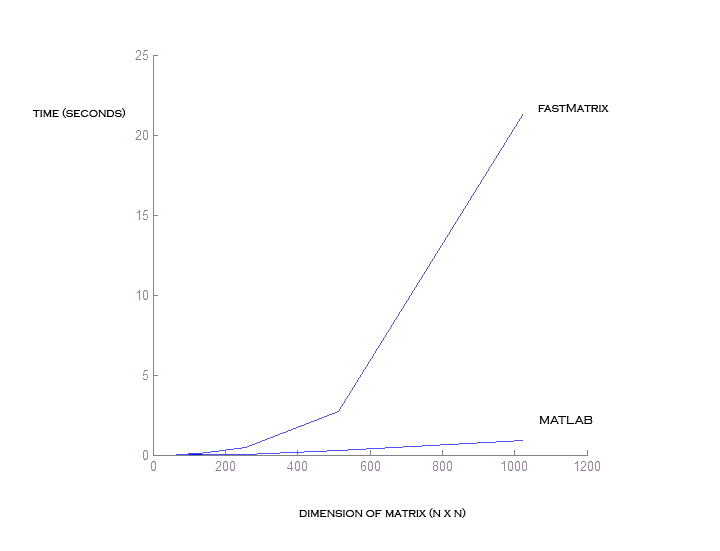
\includegraphics[scale=0.5]{./test_results/LU_decomp_np_vs_MATLAB.png}

LU factorization without pivoting on a random matrix was timed on a
Pentium M 1.6 Ghz machine. Results are $\theta(n^3)$, and clearly do
not compare well to MATLAB which uses an adapted form of the LAPACK
routines w/ partial pivoting.

\newpage

\subsection{QR factorization}

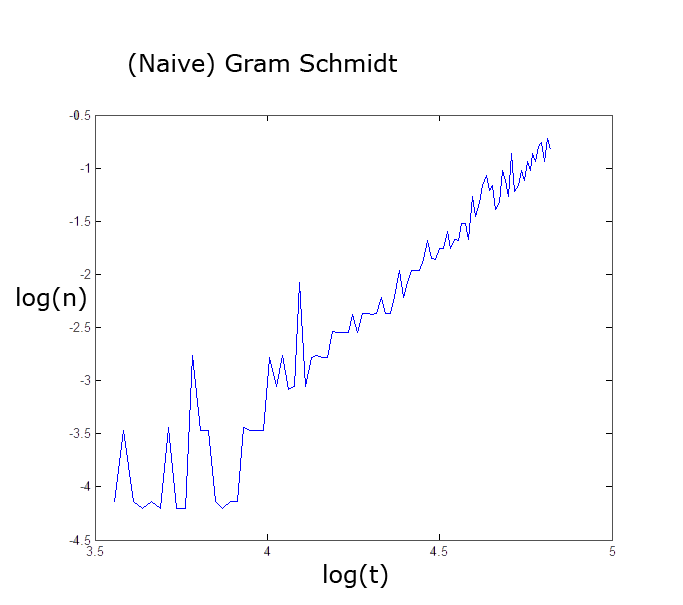
\includegraphics[scale=0.5]{./test_results/naive_gramschmidt.png}

Performance characteristic graph for QR factorization using
Householder transformations. Naive implementation is approximately
$n^{3}$.


\newpage

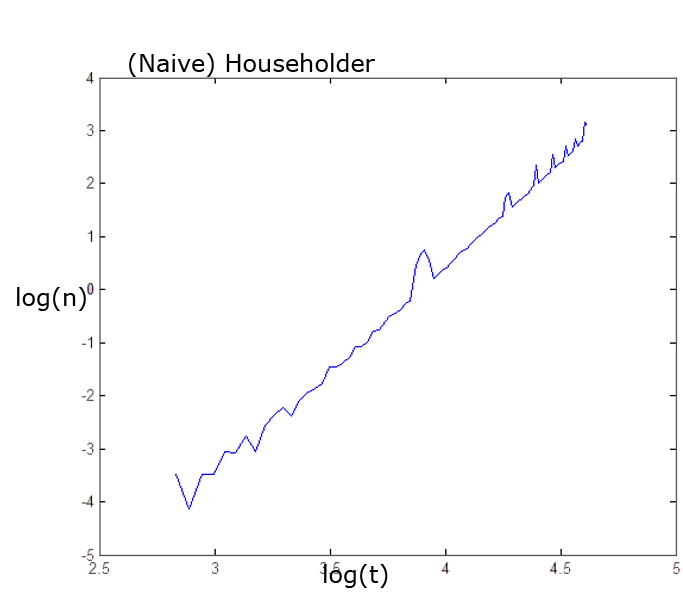
\includegraphics[scale=0.5]{./test_results/naive_householder.png}

Performance characteristic graph for QR factorization using
Householder transformations. Naive implementation is approximately
$n^{4.66}$, probably due to lots of memory manipulation. An in-place
or near-in-place implementation could perform in $n^3$ time.

\newpage

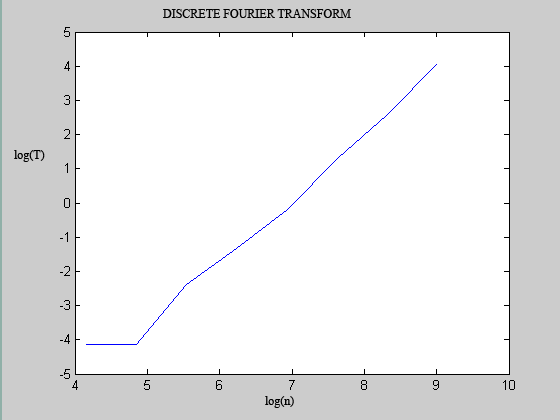
\includegraphics[scale=0.5]{./test_results/dft1.png}

Discrete Fourier Transform, as computed via a single fourier matrix
multiplication. Matrix-vector multiplication requires $\Theta(n^2)$
time steps.

\newpage

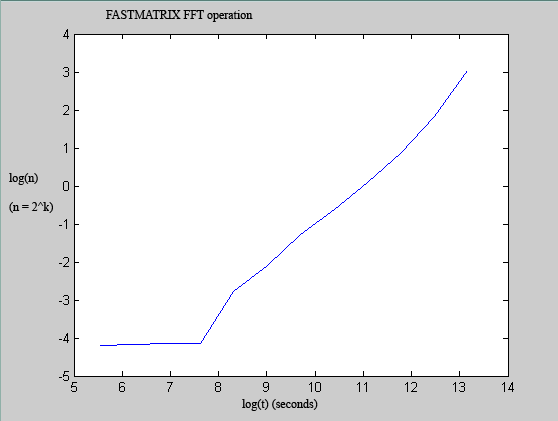
\includegraphics[scale=0.5]{./test_results/fft1.png}

Fast Fourier Transform. Implementation comes from the recursive
reference implementation provided by Corman and Rivest. Results
should be roughly $\Theta(2n \lg n)$.


\end{document}
